\documentclass[11pt]{article}
\title{\textbf{Meccano polygon diagonals}}
\author{https://github.com/heptagons/meccano/penta}
\date{}

\usepackage{../meccano}

\begin{document}

\maketitle
\begin{abstract}
We construct meccano\meccanoref polygon internal diagonals.
\end{abstract}

\section{Polygon diagonals}

\begin{figure}[H]
\centering
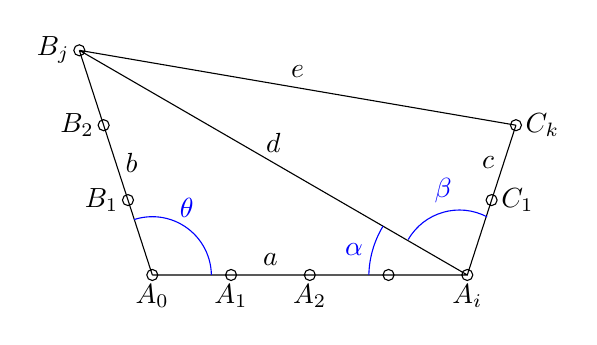
\begin{tikzpicture}
\begin{scope}[scale=1]
\begin{scope}
\draw[] (0,0) circle(2pt) node[below]{$A_i$}
-- ++(-1,0) circle(2pt)
-- ++(-1,0) circle(2pt) node[below]{$A_2$}
-- node[above]{$a$} ++(-1,0) circle(2pt) node[below]{$A_1$}
-- ++(-1,0) circle(2pt) node[below]{$A_0$}
-- ++(108:1) circle(2pt) node[left]{$B_1$}
-- node[right]{$b$} ++(108:1) circle(2pt) node[left]{$B_2$}
-- ++(108:1) circle(2pt) node[left]{$B_j$}
-- node[above]{$d$} (0,0)
-- ++(72:1) circle(2pt) node[right]{$C_1$}
-- node[left]{$c$} ++(72:1) circle(2pt) node[right]{$C_k$}
-- node[above]{$e$} ++(-5.545,0.951); % (-4-5*cos(72),sin(72))
\draw[blue] (-3.25,0) arc (0.75:108:0.75) node[midway,above]{$\theta$};
\draw[blue] (-1.25,0) arc (-1.25:-31:-1.25) node[midway,left]{$\alpha$};
\draw[blue] (-0.75,0.45) arc[start angle=90+60, end angle=62, radius=0.75] node[midway,above]{$\beta$};
\end{scope}
\end{scope}
\end{tikzpicture}
\caption{Meccano polygon three consecutive sides segments $a\ge\ b\ge c$
can form two diagonals $d$ and $e$.}
\label{fig:diagonals}
\end{figure}

\section{Regular polygon diagonals}

In the regular polygon all internal angles are equal to $\theta$.
From figure \ref{fig:diagonals} the polygon is regular if $\alpha + \beta = \theta$ so we have:
\begin{align}
\alpha &= \angle{A_0A_iB_j} \\
\beta  &= \angle{B_jA_iC_k} \\
\theta &= \angle{B_jA_0A_i} = \angle{A_0A_iC_k}\\
\alpha + \beta &= \theta
\end{align}

We use the cosines sum identity to express $\cos\beta$ in function of the rest of variables.
We define $u = \cos\theta$:
\begin{align}
u &\equiv \cos\theta\\
 &= \cos(\alpha + \beta)\\
 &= \cos\alpha\cos\beta - \sin\alpha\sin\beta\\
\sin\beta &= \frac{\cos\alpha\cos\beta - u}{\sin\alpha}\\
\sin^2\beta &= \frac{(\cos\alpha\cos\beta - u)^2}{\sin^2\alpha}\\
1 - \cos^2\beta &= \frac{\cos^2\alpha\cos^2\beta - 2u\cos\alpha\cos\beta + u^2}{sin^2\alpha}
\end{align}

We set $X = \cos\beta$ and rearrange the last equation to get:
\begin{align}
X^2 - 2u\cos\alpha X + u^2 - \sin^2\alpha &= 0
\end{align}
And solve the quadratic equation $AX^2 + BX + C = 0$ to get $\cos\beta$
in function of $u$ and $\alpha$:
\begin{align}
\cos\beta &= \frac{-B \pm \sqrt{B^2 - 4AC}}{2A}\nonumber\\
 &= \frac{2u\cos\alpha \pm 
 \sqrt{4u^2\cos^2\alpha - 4(u^2 -\sin^2\alpha)}}{2}\nonumber\\
 &= u\cos\alpha \pm \sqrt{u^2\cos^2\alpha - u^2 + \sin^2\alpha} \label{eq:cosbeta}
\end{align}

Now, we need to find the values of $\cos\alpha$, $\sin\alpha$ and $\cos\beta$ which
in turn need the value of $d$, all in terms of $a,b,c$ the segments of the polygon perimeter.
\\\\
For the value of $d$ we use the law of cosines:
\begin{align}
d &= \sqrt{a^2 + b^2 - 2ab\cos\theta} \nonumber\\
 &= \sqrt{a^2 + b^2 - 2abu} \label{eq:d}
\end{align}

Using the law of cosines we calculate the angles $\alpha =\angle{A_0A_iB_j}$ 
and $\beta =\angle{B_jA_iC_k}$:
\begin{align}
\cos\alpha &= \frac{a^2 + d^2 - b^2}{2ad} \nonumber\\
 &= \frac{a^2 + (a^2 + b^2 - 2abu) - b^2}{2ad}\nonumber \\
 &= \frac{a - bu}{d}\\
%
\cos\beta &= \frac{c^2 + d^2 - e^2}{2cd}\nonumber\\
 &= \frac{c^2 + (a^2 + b^2 - 2abu) - e^2}{2cd}\nonumber\\
 &= \frac{a^2 + b^2 + c^2 - e^2 - 2abu}{2cd}
\end{align}
We define new variable $f$ to simplify $\cos\beta$ to obtain:
\begin{align}
f &\equiv \frac{a^2 + b^2 + c^2 - e^2}{2} \\
\cos\beta &= \frac{f - abu}{cd}
\end{align}

We calculate $\sin^2\alpha = 1 - \cos^2\alpha$:
\begin{align}
\sin^2\alpha &= 1 - \frac{(a - bu)^2}{d^2}\nonumber\\
 &=\frac{d^2 - a^2 + 2abu - b^2u^2}{d^2}\nonumber\\
 &=\frac{(a^2 + b^2 - 2abu) - a^2 + 2abu - b^2u^2}{d^2}\nonumber\\
 &=\frac{b^2(1-u^2)}{d^2}
\end{align}

We plug the values of $\cos\alpha, \cos\beta, \sin^2\alpha$ in equation \ref{eq:cosbeta} to get:
\begin{align}
\frac{f - abu}{cd} &= \left(\frac{a - bu}{d}\right)u \pm \sqrt{
 \left(\frac{a - bu}{d}\right)^2u^2 - u^2 - \frac{b^2(1-u^2)}{d^2}
}\nonumber\\
\frac{f - abu}{c} &= (a - bu)u \pm \sqrt{(a-bu)^2u^2 - d^2u^2 - b^2(1-u^2)}\nonumber\\
f &= (ab + ac - bcu)u \pm c\sqrt{(a-bu)^2u^2 - d^2u^2 - b^2 +b^2u^2)}\nonumber\\
 &= abu + acu - bcu^2 \pm c\sqrt{a^2u^2 - 2abu^3 + b^2u^4- d^2u^2 - b^2 +b^2u^2 }
\end{align}
We define variables $m,n$ to simplify $f$, so we have:
\begin{align}
m &= abu + acu - bcu^2 \label{eq:m}\\
n &= a^2u^2 - 2abu^3 + b^2u^4- d^2u^2 - b^2 +b^2u^2 \label{eq:n}\\
f &= m + c\sqrt{n} \label{eq:f}\\
\frac{a^2 + b^2 + c^2 - e^2}{2} &= m + c\sqrt{n}\\
e^2 &= a^2 + b^2 + c^2 - 2m - 2c\sqrt{n}
\end{align}

\section{Regular pentagon diagonals}

For the regular pentagon we have $u = \cos\theta = \cos(3\pi/5)$:
\begin{align}
u &= \frac{1-\sqrt{5}}{4}\\
u^2 &= \frac{3-\sqrt{5}}{8}\\
u^3 &= \frac{2-\sqrt{5}}{8}\\
u^4 &= \frac{7-3\sqrt{5}}{32}
\end{align}

We plug the value of pentagon's $u$ in equation \ref{eq:d} to get $d^2$ for the pentagon:
\begin{align}
d^2 &= a^2 + b^2 - 2ab\left(\frac{1-\sqrt{5}}{4}\right)\nonumber\\
 &= \frac{4a^2 + 4b^2 - 2ab + 2ab\sqrt{5}}{4}
\end{align}
We define variables $d_1,d_2$ to simplify the previous equation:
\begin{align}
d_1 &= 4a^2 + 4b^2 - 2ab\\
d_2 &= 2ab\\
d^2 &= \frac{d_1 + d_2\sqrt5}4 \label{eq:d-penta}
\end{align}


We plug the values of pentagon's $u,u^2,u^3,u^4$ in equations \ref{eq:m} and \ref{eq:n}
to get pentagon's $m,n$:
\begin{align}
m &= ab\left(\frac{1-\sqrt5}4\right)
 + ac\left(\frac{1-\sqrt5}4\right)
 - bc\left(\frac{3-\sqrt5}8\right)\nonumber\\
 &= \frac{2ab - 2ab\sqrt5 + 2ac - 2ac\sqrt5 - 3bc + bc\sqrt5}8\nonumber\\
 &= \frac{2ab + 2ac - 3bc + (bc -2ab - 2ac)\sqrt5}8\\
%
n &= a^2\left(\frac{3-\sqrt5}8\right)
 - 2ab\left(\frac{2-\sqrt5}8\right)
 + b^2\left(\frac{7-3\sqrt5}32\right)
 - d^2\left(\frac{3-\sqrt5}8\right)
 - b^2
 + b^2\left(\frac{3-\sqrt5}8\right)\nonumber\\
 &= \frac{
 12a^2 - 4a^2\sqrt5 -16ab+8\sqrt5 +7b^2-3b^2\sqrt5 -12d^2+4d^2\sqrt5 -32b^2
 +12b^2-4b^2\sqrt5
 }{32}\nonumber\\
 &= \frac{12a^2 - 16ab - 13b^2 - 12d^2 + (-4a^2 + 8 - 3b^2 + 4d^2 - 4b^2)\sqrt5}{32}
\end{align}

We substitute $d^2$ of last equation with equation \ref{eq:d-penta} value in terms of $d_1,d_2$
to isolate correctly $\sqrt5$ factors:
\begin{align}
n &= \frac{
 12a^2 - 16ab - 13b^2 - 3(d_1 + d_2\sqrt5)
 + (-4a^2 + 8 - 3b^2 + (d_1 + d_2\sqrt5) - 4b^2)\sqrt5
}{32} \nonumber\\
 &= \frac{
 12a^2 - 16ab - 13b^2 - 3d_1 + 5_d2
 + (-4a^2 + 8 - 3b^2 + d_1 - 3d_2)\sqrt5
 }{32}
\end{align}

We define $m1,m2,n1,n2$ to simplify previous formulas of $m,n$ to obtain:
\begin{align}
m_1 &= 2ab + 2ac - 3bc \\
m_2 &= bc -2ab - 2ac\\
n_1 &= 12a^2 - 16ab - 13b^2 - 12d^2\\
n_2 &= -4a^2 + 8 - 3b^2 + 4d^2 - 4b^2
\end{align}

\subsection{Regular pentagon height}

In the regular pentagon the height $H$ is the distance from one side of length a to the opposite vertex:
\begin{align}
H &= \frac{\sqrt{5+2\sqrt{5}}}{2}a
\end{align}
For the height to occur (coincident with diagonal $e$) we need $a = b = c/2$.
We calculate first the diagonal $d$ plugin $a=b$ in equation \ref{eq:d-penta}:
\begin{align}
d_{a=b} &= \frac{\sqrt{4a^2 + 4a^2 - 2a^2 + 2a^2\sqrt{5}}}{2}\nonumber\\
 &= \frac{\sqrt{6-2\sqrt{5}}}{2}a\nonumber\\
 &= \frac{\sqrt{5}-1}{2}a
\end{align}


\end{document}
